\chapter{False Sharing}
\label{app:false_sharing}

In the context of this thesis, memory is considered to be split into memory
elements (see Definition~\ref{def:memoryelement}), with a size corresponding to
that of a cache line. This means that the minimal size that can be addressed
(i.e.~a byte) is that of a cache line. Realistically however, cache lines are
generally able to hold 32, 64, 128 bytes. The false sharing issue stems from the
fact that cache lines are the size of the blocks being loaded into caches, so
loading any address within a block of that size loads data for other addresses.

\begin{figure}[hbt!]
\begin{subfigure}[t]{\textwidth}
\resizebox{\linewidth}{!}{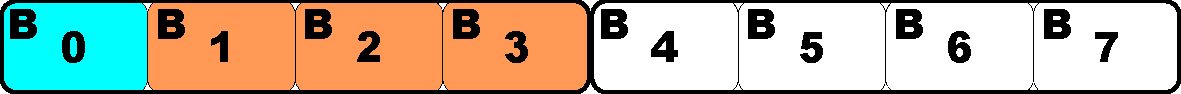
\includegraphics{\chapterdirectory/figure/false_sharing_0.pdf}}
\caption{Default Data Placement}
\label{fig:false_sharing:default}
\end{subfigure}
\begin{subfigure}[t]{\textwidth}
\resizebox{\linewidth}{!}{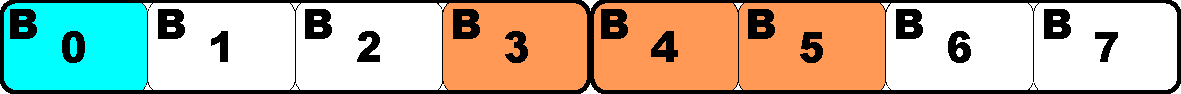
\includegraphics{\chapterdirectory/figure/false_sharing_1.pdf}}
\caption{Insufficient Padding}
\label{fig:false_sharing:wrong_padding}
\end{subfigure}
\begin{subfigure}[t]{\textwidth}
\resizebox{\linewidth}{!}{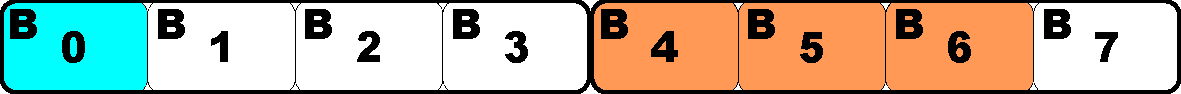
\includegraphics{\chapterdirectory/figure/false_sharing_2.pdf}}
\caption{Data Placement Without False Sharing}
\label{fig:false_sharing:right_padding}
\end{subfigure}
\caption{Examples of Data Placements}
\label{fig:false_sharing:paddings}
\end{figure}

To understand what false sharing is, let us consider an architecture with two
cores, $\texttt{Core}_0$ and $\texttt{Core}_1$, both having their own cache,
$\texttt{Cache}_0$ and $\texttt{Cache}_1$, with cache coherence being active.
Let us consider that these caches have cache lines with a size of
contain 4 bytes, and that both cores are currently making numerous memory
accesses to one variable each, $\texttt{Var}_0$ and $\texttt{Var}_1$.
$\texttt{Var}_0$ is 1 byte long, and $\texttt{Var}_1$ is 3 bytes long.
Figure~\ref{fig:false_sharing:paddings} shows how both variables could be
placed in memory.

Caches access whole cache lines, meaning that accessing any address between
0 and 3 inclusive leads to the transfer of all bytes in this interval into the
cache.

The placement shown in Figure~\ref{fig:false_sharing:default} corresponds to
putting $\texttt{Var}_0$ at address 0, and $\texttt{Var}_1$ at address 1. This
is the most memory efficient solution. However, this configuration, a cache
accessing to either variable also performs an access to the other variable. This
is not obvious from a program's point of view, as the two variables have
separate addresses. The effect is that cache coherence has to be maintained
between both caches upon any operation performed on either variables, despite
the fact that each core never actually addresses the other core's variable. To
avoid this very costly and unrequited cache coherence, the solution is to add
padding: place the variables so that a cache accessing one does not accesses the
other.

Utilities to ensure a given memory block is allocated in memory with sufficient
padding for a given cache line size are available in C/C++ (for dynamic memory
allocation) and in popular compilers (for static memory allocations). Since this
alignment is not done by default, this requires that the programmer is aware of
the false sharing issue. Furthermore, it also requires the cache line be known
at compilation time, which is an issue for portable programs.
Figure~\ref{fig:false_sharing:wrong_padding} shows a placement in which an
insufficient padding has been used. By placing $\texttt{Var}_1$ at address 3,
the amount of data transfers is further increased: not only is the false sharing
issue still there, but now two cache lines have to be accessed when accessing
$\texttt{Var}_1$.

Figure~\ref{fig:false_sharing:right_padding} shows a padding corresponding to
$\texttt{Var}_1$ being placed at address 4, which ensures that accessing either
variable only transfers a single cache line and that no false sharing can occur
between these two variables.
